%%%%%%%%%%%%%%%%%%%%%%%%%%%%%%%%%%%%%%%%%%%%%%%%%%%%%%%%%%%%%%%%%%%%%%%
% Info
%%%%%%%%%%%%%%%%%%%%%%%%%%%%%%%%%%%%%%%%%%%%%%%%%%%%%%%%%%%%%%%%%%%%%%%
% Author: Louis Pahlavi
% Email:  louis.pahlavi@mail.utoronto.ca

% This is my personal resume. All the document setup is made inside the
% "Resume" template.

%%%%%%%%%%%%%%%%%%%%%%%%%%%%%%%%%%%%%%%%%%%%%%%%%%%%%%%%%%%%%%%%%%%%%%%
% General setup
%%%%%%%%%%%%%%%%%%%%%%%%%%%%%%%%%%%%%%%%%%%%%%%%%%%%%%%%%%%%%%%%%%%%%%%
\documentclass{ResumeTemplate}
\usepackage{tabularx}
\usepackage{graphicx}

% Bibliography
\usepackage{biblatex}
\addbibresource{references.bib}

%%%%%%%%%%%%%%%%%%%%%%%%%%%%%%%%%%%%%%%%%%%%%%%%%%%%%%%%%%%%%%%%%%%%%%%
% Document
%%%%%%%%%%%%%%%%%%%%%%%%%%%%%%%%%%%%%%%%%%%%%%%%%%%%%%%%%%%%%%%%%%%%%%%
\begin{document}

	\fontsize{10}{12}\selectfont
	
	%%%%%%%%%%%%%%%%%%%%%%%%%%%%%%%%%%%%%%%%%%%%%%%%%%%%%%%%%%%%%%%%%%%
	% Title and headers
	%%%%%%%%%%%%%%%%%%%%%%%%%%%%%%%%%%%%%%%%%%%%%%%%%%%%%%%%%%%%%%%%%%%

	\centering\myname{Louis L. W. D. Pahlavi}
	~

	\raggedright\begin{minipage}[c]{0.65\linewidth} 

		%%%%%%%%%%%%%%%%%%%%%%%%%%%%%%%%%%%%%%%%%%%%%%%%%%%%%%%%%%%%%%%%%%%
		% Technical Skills
		%%%%%%%%%%%%%%%%%%%%%%%%%%%%%%%%%%%%%%%%%%%%%%%%%%%%%%%%%%%%%%%%%%%
		
		\section{TECHNICAL SKILLS}
		
		\noindent\begin{tabularx}{\linewidth}{>{\bfseries}lX}
		   Build tools     & Makefile, CMake \\
		   Version control & Git \\
		   Platforms       & Linux, Raspberry Pi, Arduino \\
		   Libraries       & Boost, QT, CVX, Tensorflow \\
		   Theory          & Control theory and robotics, Networking, Optimization, Algorithms, Machine learning
		\end{tabularx}

		%%%%%%%%%%%%%%%%%%%%%%%%%%%%%%%%%%%%%%%%%%%%%%%%%%%%%%%%%%%%%%%%%%%
		% Education
		%%%%%%%%%%%%%%%%%%%%%%%%%%%%%%%%%%%%%%%%%%%%%%%%%%%%%%%%%%%%%%%%%%%
		\section{EDUCATION}
		
		\datedsubsection{University of Toronto, BASc in Computer Engineering}{September 2014--April 2019}
		\workitemsfour
		{Minor in Robotics and Mechatronics}
		{Final Project: \textit{Distributed Formation Control of a Swarm of Unicycles}}
		{16 month internship between third and fourth years of studies}
		{Latest term 92.1\% average (ranked 4 out of 173), 3.86/4.00 CGPA}
	
		%%%%%%%%%%%%%%%%%%%%%%%%%%%%%%%%%%%%%%%%%%%%%%%%%%%%%%%%%%%%%%%%%%%
		% Awards and Scholarships
		%%%%%%%%%%%%%%%%%%%%%%%%%%%%%%%%%%%%%%%%%%%%%%%%%%%%%%%%%%%%%%%%%%%
		\section{SCHOLARSHIPS AND AWARDS}	
		\begin{itemize}[noitemsep, leftmargin=*]
			\item \textbf{Applied Science and Engineering Dean's Honours List} \hfill 2014--Present
			\item \textbf{Gordon R. Slemon Scholarship} \hfill 2016
			% \item \textbf{University of Toronto International Exchange Bursary} \hfill 2016
			\item \textbf{University of Toronto Centre for International Exchange Award} \hfill 2016
			\item \textbf{Royal Canadian Air Cadet Power Pilot Scholarship} \hfill 2014
			% \item \textbf{Royal Canadian Air Cadet Glider Pilot Scholarships} \hfill 2013\vspace*{-\baselineskip}
		\end{itemize}

	\end{minipage}
	\hspace{0.01\linewidth}
	\noindent\begin{minipage}[c]{0.33\linewidth}
		\centering

		%%%%%%%%%%%%%%%%%%%%%%%%%%%%%%%%%%%%%%%%%%%%%%%%%%%%%%%%%%%%%%%%%%%
		% Technical Skills
		%%%%%%%%%%%%%%%%%%%%%%%%%%%%%%%%%%%%%%%%%%%%%%%%%%%%%%%%%%%%%%%%%%%
		% 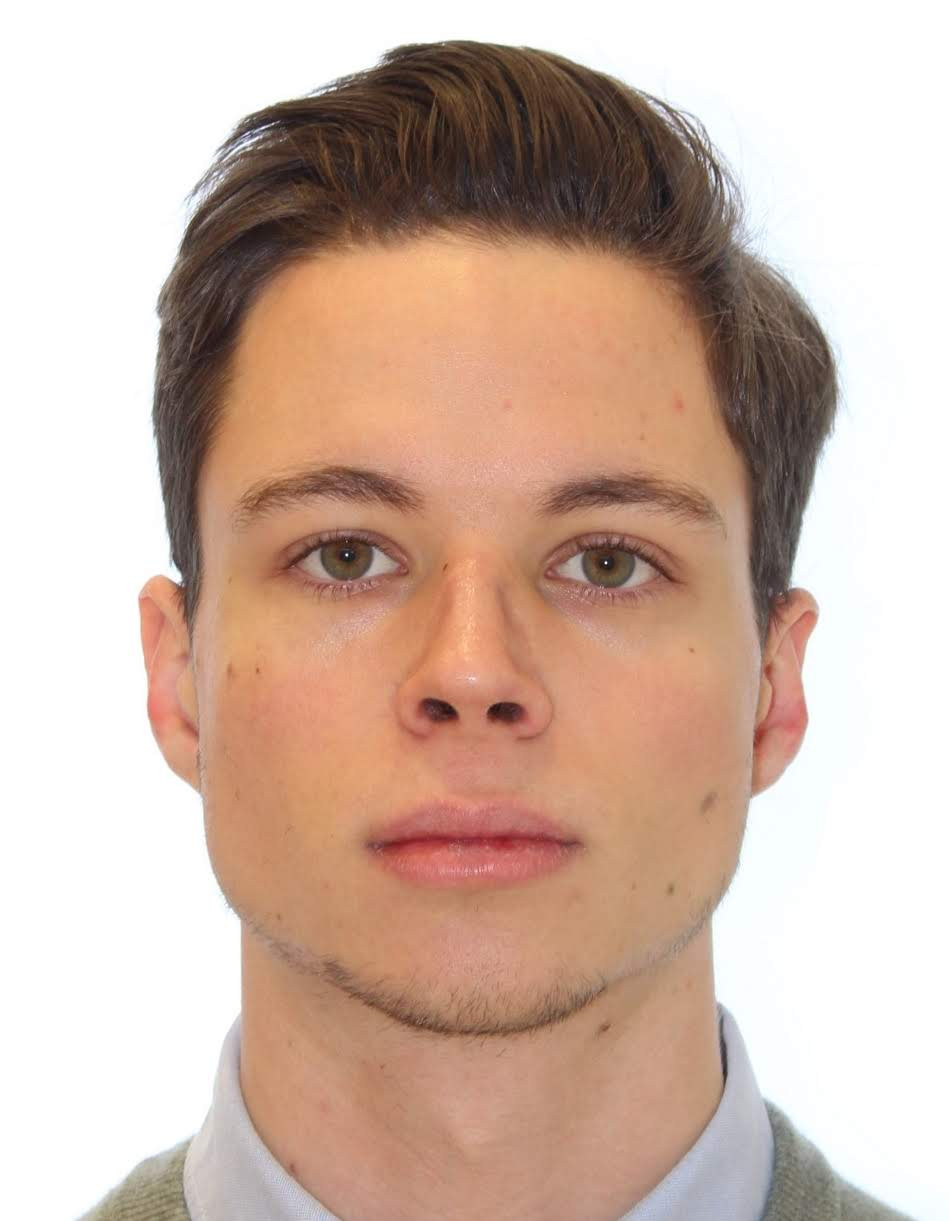
\includegraphics[width=0.5\linewidth]{me}

		%%%%%%%%%%%%%%%%%%%%%%%%%%%%%%%%%%%%%%%%%%%%%%%%%%%%%%%%%%%%%%%%%%%
		% Personal details
		%%%%%%%%%%%%%%%%%%%%%%%%%%%%%%%%%%%%%%%%%%%%%%%%%%%%%%%%%%%%%%%%%%%
		
		\section{PERSONAL DETAILS}
		
		\noindent\begin{tabularx}{\linewidth}{lX}
		   \textbf{Nationality:} & French, Canadian
		\end{tabularx}
		
		\noindent\begin{tabularx}{\linewidth}{lX}
		   % \passportsymbol & French, Canadian \\
		   \emailsymbol    &  louis.pahlavi@mail.utoronto.ca\\
		   \phonesymbol    & +1 (647) 909-5487 \\
		   \mailsymbol     & 106 Wineva Ave, Toronto, ON, M4E 2T2, Canada \\
		   \homepagesymbol & \href{https:\\lpahlavi.github.io}{lpahlavi.github.io}
		\end{tabularx}
		
		% \section{NATIONALITY}
		
		% French, Canadian

		%%%%%%%%%%%%%%%%%%%%%%%%%%%%%%%%%%%%%%%%%%%%%%%%%%%%%%%%%%%%%%%%%%%
		% Technical Skills
		%%%%%%%%%%%%%%%%%%%%%%%%%%%%%%%%%%%%%%%%%%%%%%%%%%%%%%%%%%%%%%%%%%%
		\section{LANGUAGES}

		\cvskill{English}{5}
		\cvskill{French}{5}
		\cvskill{Italian}{4}
		\cvskill{German}{3}
		\cvskill{Czech}{1}

		%%%%%%%%%%%%%%%%%%%%%%%%%%%%%%%%%%%%%%%%%%%%%%%%%%%%%%%%%%%%%%%%%%%
		% Technical Skills
		%%%%%%%%%%%%%%%%%%%%%%%%%%%%%%%%%%%%%%%%%%%%%%%%%%%%%%%%%%%%%%%%%%%
		\section{PROGRAMMING LANGUAGES}

		\cvskill{C/C++}{5}
		\cvskill{Python}{5}
		\cvskill{MATLAB}{4}
		\cvskill{Java}{2}
	\end{minipage}
	
	%%%%%%%%%%%%%%%%%%%%%%%%%%%%%%%%%%%%%%%%%%%%%%%%%%%%%%%%%%%%%%%%%%%
	% Education
	%%%%%%%%%%%%%%%%%%%%%%%%%%%%%%%%%%%%%%%%%%%%%%%%%%%%%%%%%%%%%%%%%%%
	\section{RESEARCH AND INDUSTRY EXPERIENCE}
	
	\position{Systems and Control Engineering Intern}{May 2017--August 2018}{\href{https://veritystudios.com/}{Verity Studios AG}}{Z{\"u}rich, Switzerland}

	\workitemsthree
	{Worked on improving the onboard control algorithms of swarms of quadcopters implemented in C++.}
	{Evaluated and characterized flight performance and effectiveness of calibration routines using Python.}
	{Serviced entertainment drone show systems overseas and oversaw flight operations for several weeks.}
	
	\position{Researcher}{May 2016--August 2016}{\href{http://www.lbb.ethz.ch/}{ETH Z{\"u}rich Laboratory for Biosensors and Bioelectronics}}{Z{\"u}rich, Switzerland}
	
	\workitemstwo
	{Developed the control and image processing software for a biosensor measuring protein interactions.}
	{Created a Graphical User Interface using Qt to control the actuators and interface them with various sensors.}
	
	\position{Researcher}{May 2015--September 2015}{\href{http://www.waves.utoronto.ca/prof/svhum/}{University of Toronto Reconfigurable Antenna Laboratory}}{Toronto, Canada}

	\workitemstwo
	{Designed and simulated the early prototypes of a deployable antenna mounted on the NORSAT-2 maritime communications satellite (launched in 2017) in collaboration with the European Space Agency.}
	{Created a MATLAB simulation to model a satellite's orbit and predict antenna radiation intensity on the surface of the Earth. Worked on antenna synthesis to find an antenna array for a given desired coverage area.}
	
	%%%%%%%%%%%%%%%%%%%%%%%%%%%%%%%%%%%%%%%%%%%%%%%%%%%%%%%%%%%%%%%%%%%
	% Projects and Teaching
	%%%%%%%%%%%%%%%%%%%%%%%%%%%%%%%%%%%%%%%%%%%%%%%%%%%%%%%%%%%%%%%%%%%
	\section{PROJECTS AND TEACHING}
	
	\position{Capstone Team Lead}{September 2018--April 2019}{\href{https://www.engineering.utoronto.ca/}{University of Toronto Faculty of Engineering}}{Toronto, Canada}

	\workitemsthree
	{Implementing a fully distributed algorithm for the formation control of a swarm of wheeled robots in C++.}
	{Built and tested the communication interfaces between onboard modules and C++ and Python applications.}
	{Developed a Python simulation framework to test and tune the control algorithms. }
	
	% \position{Teaching Assistant}{September 2016--December 2016}{\href{https://www.engineering.utoronto.ca/}{University of Toronto Faculty of Engineering}}{Toronto, Canada}

	% \workitemsone
	% {Taught APS100 -- 'Orientation to Engineering' to first year Electrical and Computer Engineering students.}
	
	\position{Wireless Communications Lead}{September 2014--June 2016}{\href{https://www.utat.ca/space-systems/}{University of Toronto Aerospace Team (Space Systems)}}{Toronto, Canada}

	\workitemstwo
	{Designed, built and tested the antenna and communication module PCB, on a student-built nano-satellite.}
	{Presented our design at several Product Design Reviews and the Critical Design Review in Vancouver.}

	% \position{Ground School Instructor}{September 2014--January 2015}{330 Danforth Tech Royal Canadian Air Cadet Squadron}{Toronto, Canada}
	
	% \workitemsone
	% {Coordinated and taught the pilot ground school course at 330 Danforth Tech Royal Canadian Air Cadet Squadron.}

\end{document}